%%
%% PPLP Final Report -- ACM sigconf (2-column) format
%% Privacy-Preserving Link Prediction
%%
%% This is the final report. It preserves the midterm content verbatim
%% (Sections 1--4) and extends it with Sections 5--11 describing what we
%% actually built.
%%
\documentclass[sigconf]{acmart}

\usepackage{graphicx}
\usepackage{tikz}
\usetikzlibrary{positioning,arrows.meta,calc}
\usepackage{booktabs}

\AtBeginDocument{%
  \providecommand\BibTeX{{Bib\TeX}}}

\setcopyright{acmlicensed}
\copyrightyear{2026}
\acmYear{2026}
\acmDOI{10.1145/XXXXXXX.XXXXXXX}
\acmConference[CSDS 356/456]{Project Report (Final)}{2026}{Cleveland, OH}
\settopmatter{printacmref=false}

\begin{document}

\title{PPLP: Privacy-Preserving Link Prediction}

\author{Kaleb Kim, Wiam Skakri, Carson Whitehouse, Jonah Lorenzo}
\author{Kent Manion, and Aidan Bugayong}
\affiliation{%
  \institution{Case Western Reserve University}
  \city{Cleveland}
  \state{Ohio}
  \country{USA}
}
\renewcommand{\shortauthors}{Kim et al.}

\begin{abstract}
Distributed link prediction over multiple graphs can improve accuracy but raises privacy concerns. We describe a Python library for \emph{privacy-preserving link prediction} (PPLP): two parties compute link-prediction scores over the union of their graphs without revealing graph structure. The library implements the protocol of Demirag et al.~\cite{Demirag2022} on top of OpenMined PSI~\cite{openminedpsi} (substituted for the originally planned ultra-fast PSI of Ling et al.~\cite{ling2025ultrafast} for portability), supports Common Neighbors and Jaccard, and is exposed as a Python API, a CLI server, and a Streamlit dashboard. The principal design choice is to recast the paper's symmetric peer protocol as an asymmetric server--client service, enabling a data-as-a-service deployment but introducing a new threat surface: adaptive queries against a fixed server graph. We present microbenchmarks ($\le 0.6$ s per query at neighborhood sizes of 1\,000), a sequence-level breakdown of the HTTP API, an end-to-end demonstration over four datasets, and the residual threat model.
\end{abstract}

\keywords{link prediction, private set intersection, homomorphic encryption, distributed graphs, privacy}

\maketitle

%=============================================================================
\section{Problem Statement and Literature Search}
%=============================================================================

\subsection{Link Prediction}
Link prediction aims to discover unobserved or latent connections between nodes in a graph~\cite{liben-nowell2007link}. Given a snapshot of a network at time $t$, the goal is to predict which edges will appear by a future time $t'$ using structural information (e.g., proximity measures or graph neural networks). Applications include social networks, e-commerce, telecommunications, fraud and financial crime detection, and bioinformatics explored in a later section.

Link prediction is typically performed on a single local graph. Distributed link prediction considers the setting where two or more parties hold related graphs (e.g., overlapping node sets or the same domain). Merging these graphs can yield more accurate predictions, but sharing raw graph data raises privacy risks: identity disclosure, link disclosure, and attribute disclosure. We therefore focus on privacy-preserving link prediction (PPLP): multiple data holders collaboratively compute link-prediction scores over their combined graph \emph{without} revealing their private graph structure to each other (Figure~\ref{fig:motivation}).

\begin{figure*}
  \centering
  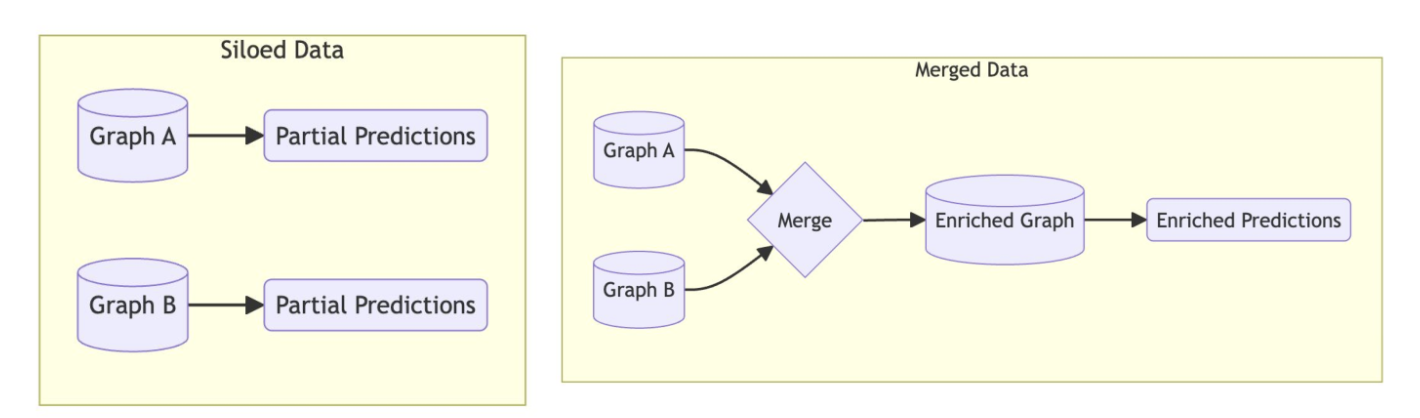
\includegraphics[width=\textwidth]{figures/link_prediction.png}
  \Description{Two diagrams side by side. Left: siloed data showing Graph A and Graph B each producing separate partial predictions. Right: merged data showing Graph A and Graph B combined via a merge step into an enriched graph yielding enriched predictions.}
  \caption{Siloed vs.\ merged data. Each party independently produces only partial predictions (left), whereas merging graphs yields an enriched, more accurate result (right), at the cost of privacy without PPLP.}
  \label{fig:motivation}
\end{figure*}

\subsection{Related Work}

Liben-Nowell and Kleinberg~\cite{liben-nowell2007link} formalize the link-prediction problem using only network topology (no node attributes) and conduct a study of proximity-based measures on co-authorship networks. Their analysis establishes common neighbors, Jaccard, and Adamic--Adar as the foundation for topologically driven link prediction that significantly outperform random baselines. This topology framing allows for a set-based approach that enables compatibility with Private Set Intersection (PSI).

Ayday et al.~\cite{Demirag2022} give a two-party protocol in which each party holds a graph; they compute \emph{common neighbor} counts over the union of both graphs using a notably small number of private set intersection (PSI) and additively homomorphic encryption calls. The common-neighbor count is expressed as local terms plus crossover terms minus overlaps such that only intersection sizes rather than neighbor sets are revealed. They also discuss a heavier homomorphic variant to reduce intermediate leakage where neither party can learn the intermediate intersection sizes before the final output is assembled. Their threat model assumes semi-honest (honest-but-curious) adversaries and no trusted third party, which is realistic for competitive or regulated settings such as cross-institutional healthcare.

PSI is the core cryptographic primitive enabling the PPLP protocol, as it lets two parties compute the intersection of their sets while revealing only the result. Chen et al.~\cite{chen2017fast} give a high-performance PSI protocol from fully homomorphic encryption (FHE) with communication complexity $O(N_{\text{small}} \cdot \log N_{\text{large}})$. Lattice-based FHE~\cite{gentry2009lattice} made such protocols practical by bootstrapping and resolving the noise problem with a decryption circuit. Ling et al.~\cite{ling2025ultrafast} propose an ultra-fast PSI from efficient Oblivious Key-Value Stores (OKVS) and Vector Oblivious Linear Evaluation (VOLE), with $O(n)$ communication and low encoding redundancy (on the order of 1\%), making it significantly faster in practice for large sets than FHE-based PSI. We plan to use it for our Python library implementation due to its linear communication cost and lower overhead.

\subsection{Motivating Use Cases}
Applications span several domains, each presenting distinct graph structures and privacy considerations.

Social networks: PPLP powers friend recommendations by surfacing latent connections between users across a network snapshot. Sharing edge data across multiple networks risks re-identifying pseudonymous users through structural patterns.

E-commerce: PPLP drives product recommendation by predicting new edges in a bipartite user-product graph built from purchase and interaction history. Multiple retailers may hold overlapping customer bases, but sharing purchase graphs exposes proprietary customer behavior data.

Telecommunications: PPLP enables targeted advertising by modeling call or message patterns among users. Call graphs reveal associations and routines so sharing them across carriers raises attribute and link disclosure concerns.

Bioinformatics: PPLP allows for merging of Electronic Health Records (EHR) with clustering graphs to allow better research and predictions of patient diagnosis, disease spread, drug interactions, and more as derived from clinical and experimental data.

Financial networks: PPLP supports fraud detection by identifying suspicious latent connections between accounts at different institutions through intermediary accounts, which is a marker for money-laundering. Raw graph sharing is largely prohibited by financial privacy regulation, so this could allow banks to more completely observe the transaction subgraph of a potentially criminal organization.

%=============================================================================
\section{Planned Methods}
%=============================================================================

\subsection{Link-Prediction Measures}
We will support at least one of the following proximity-based measures, which can be expressed using set operations over neighbor sets and thus combined with PSI.

\begin{itemize}
  \item \textbf{Common Neighbors (CN):} For nodes $u$ and $v$, $\text{CN}(u,v) = |N(u) \cap N(v)|$. More common neighbors imply higher link likelihood.
  \item \textbf{Jaccard:} $\frac{|N(u) \cap N(v)|}{|N(u) \cup N(v)|}$, which accounts for the relative overlap.
  \item \textbf{Adamic--Adar (AA):} $\sum_{w \in N(u) \cap N(v)} \frac{1}{\log |N(w)|}$, emphasizing common neighbors with lower degree.
\end{itemize}

\subsection{Threat Model}
\label{sec:midterm-threat-model}
We assume a two-party, semi-honest (honest-but-curious) adversary model. Both Alice and Bob execute the protocol steps faithfully; they do not deviate, send malformed inputs, or abort early. However, each party attempts to infer as much as possible about the other's private graph from the protocol messages they legitimately receive. Each party enters the protocol knowing its own graph in full, the set of candidate node pairs for which link scores are being computed, and the public protocol specification.

The PSI calls expose only the \emph{sizes} of intersection sets (e.g., $|I_{A+B}|$ and the crossover intersection sizes), not the sets themselves. The final output, i.e., the common-neighbor count for each candidate pair, is learned by both parties. Neither party should learn the other's raw neighbor sets: Alice must not learn $N_B(u)$ for any node $u$, and Bob must not learn $N_A(u)$.

The basic protocol leaks intermediate intersection sizes, which may allow inferences about the other party's graph degree distribution. Ayday et al.\ propose a heavier homomorphic variant that eliminates even this leakage; we plan to explore this as an extension. Malicious adversaries, party collusion, side-channel attacks, and settings with more than two parties are out of scope for the initial prototype.

\subsection{Two-Party Common Neighbors via PSI}
Following Ayday et al., for two parties Alice (graph $G_A$) and Bob (graph $G_B$), the common-neighbor count for a candidate pair $(A,E)$ can be decomposed into the following local and crossover terms. Figure~\ref{fig:graph-union} shows a concrete example where Alice holds $G_A$ over nodes $\{A,B,C,D,E,G,H\}$ and Bob holds $G_B$ over nodes $\{A,B,C,D,E,K,F\}$, with the two graphs sharing the node subset $\{A,B,C,D,E\}$.
\begin{itemize}
  \item Local intersections: $I_A(A,E) = N_A(A) \cap N_A(E)$ and $I_B(A,E) = N_B(A) \cap N_B(E)$ (each party computes locally).
  \item Crossover terms: e.g., $N_A(A) \setminus I_A$ with $N_B(E) \setminus I_B$, etc., which require PSI so that only intersection sizes (or masked sets) are revealed.
\end{itemize}
The total $|\text{CN}(A,E)|$ is then obtained as $|I_A| + |I_B| - |I_A \cap I_B|$ plus the contributions from the crossover PSI results (e.g., $|I_{A+B}|$ and the sizes of the privately computed crossover intersections). The protocol uses a small, fixed number of PSI calls per candidate pair. Figures~\ref{fig:applying-psi} and~\ref{fig:cn-result} walk through this computation on the running example.

\begin{figure*}
  \centering
  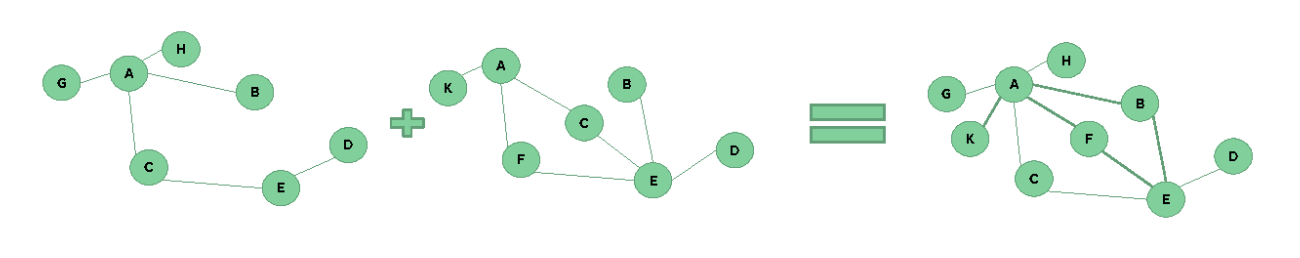
\includegraphics[width=\textwidth]{figures/distributed_link_prediction.png}
  \Description{Three graphs shown left to right with a plus sign and an equals sign between them. The left graph (Alice) has nodes A, B, C, D, E, G, H. The center graph (Bob) has nodes A, B, C, D, E, K, F. The right graph shows their union with all nodes combined.}
  \caption{Two-party graph union. Alice's graph $G_A$ (left) and Bob's graph $G_B$ (center) share overlapping node set $\{A,B,C,D,E\}$; their union (right) contains additional nodes $G$, $H$ from Alice and $K$, $F$ from Bob.}
  \label{fig:graph-union}
\end{figure*}

\begin{figure*}
  \centering
  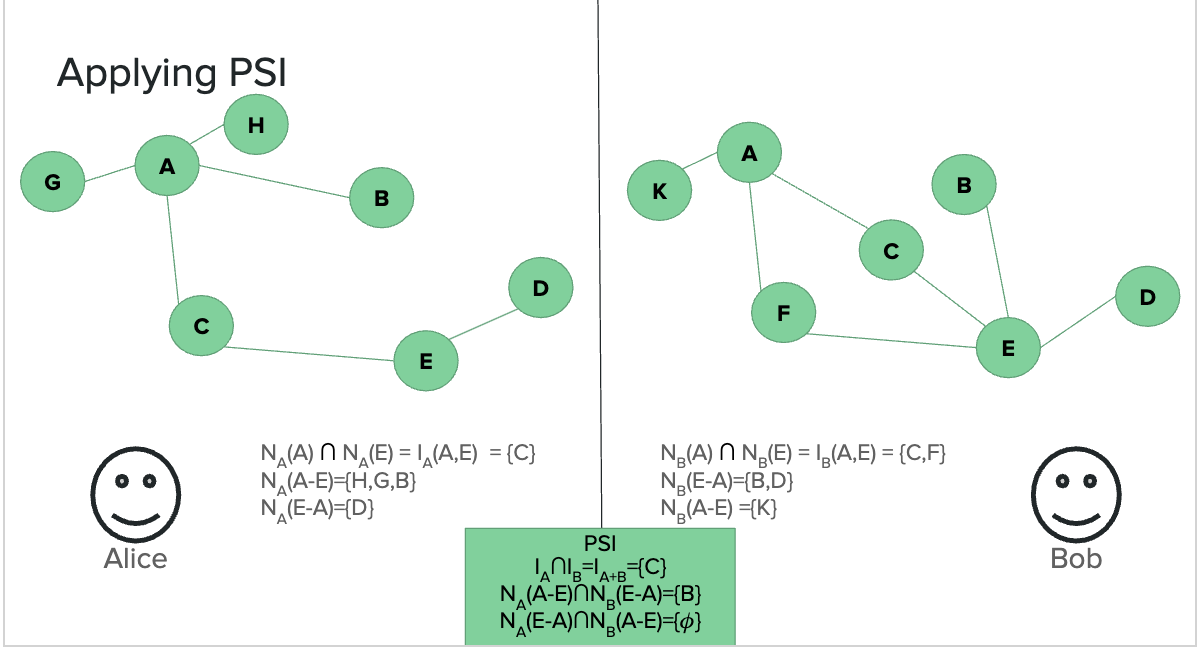
\includegraphics[width=\textwidth]{figures/applying_psi.png}
  \Description{Side-by-side diagrams of Alice's graph and Bob's graph for candidate pair (A,E). Each party's local neighbor sets and local intersections are shown below their graph. A central PSI box shows three crossover intersection results computed privately.}
  \caption{Applying PSI for candidate pair $(A,E)$. Alice and Bob first compute local intersections $I_A$ and $I_B$ independently. Three PSI calls then privately resolve the crossover terms: $I_A \cap I_B = \{C\}$, $N_A(A\text{-}E) \cap N_B(E\text{-}A) = \{B\}$, and $N_A(E\text{-}A) \cap N_B(A\text{-}E) = \emptyset$.}
  \label{fig:applying-psi}
\end{figure*}

\begin{figure*}
  \centering
  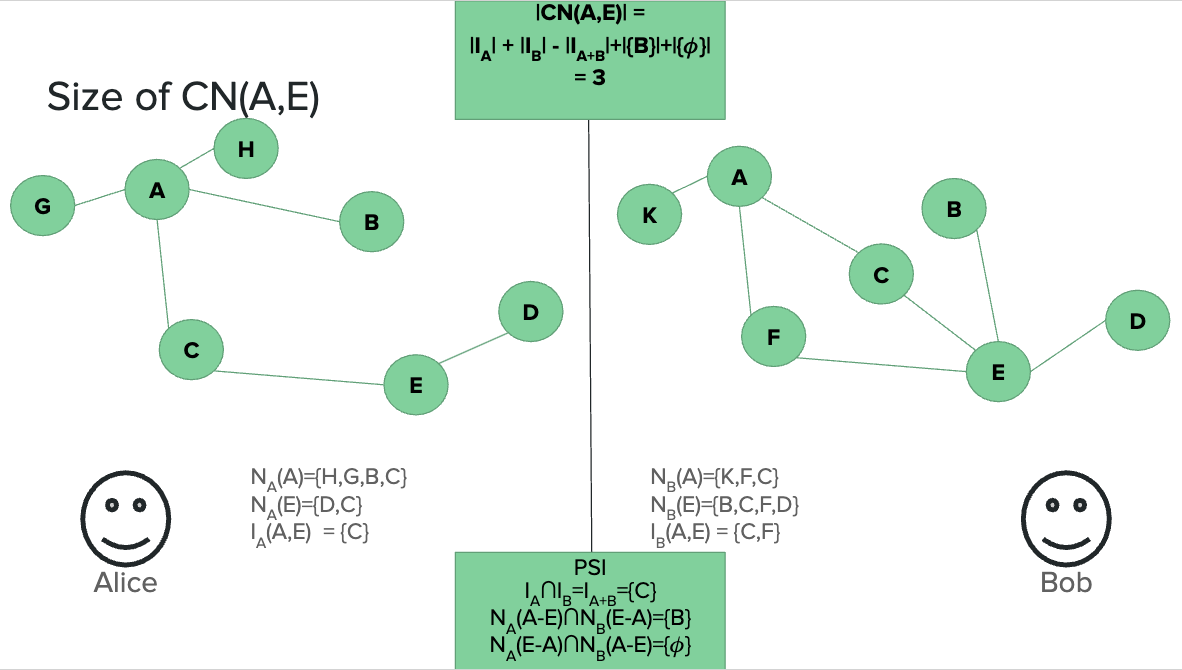
\includegraphics[width=\textwidth]{figures/size_of_cn.png}
  \Description{Alice's and Bob's graphs for pair (A,E) with all neighbor sets and local intersections listed below each graph. A top banner shows the formula |CN(A,E)| = |I_A| + |I_B| - |I_{A+B}| + |{B}| + |{phi}| = 3. A central PSI box shows the three crossover results.}
  \caption{Computing $|\text{CN}(A,E)|$. Combining local terms $|I_A|{=}1$ and $|I_B|{=}2$ with the PSI-computed crossover results yields $|\text{CN}(A,E)| = 1 + 2 - 1 + 1 + 0 = 3$.}
  \label{fig:cn-result}
\end{figure*}

\subsection{Two-Party Node Cardinalities via PSI}
Similar to Common Neighbors, two parties can find out the combined cardinalities for common nodes between the parties. Assume again that Alice (graph $G_A$) and Bob (graph $G_B$) first perform PSI on the node sets of their graphs to determine which nodes they share, then compute combined cardinalities for those shared nodes. Below are the steps to determine the combined cardinality of node $A$:
\begin{itemize}
  \item Local Cardinalities: $N_A(A)$ and $N_B(A)$ (each party computes locally).
  \item Intersection Term: $N_A(A) \cap N_B(A)$, which requires PSI so that only the intersection size (or masked set) is revealed.
\end{itemize}
The total $|N_{A+B}(A)|$ is then obtained as $|N_A(A)| + |N_B(A)| - |N_A(A) \cap N_B(A)|$. The protocol uses a single PSI call per node, although an additional PSI call is required to determine which nodes are available to both parties.

\subsection{Privacy Primitives}
\begin{itemize}
  \item \textbf{Private Set Intersection (PSI):} Core primitive to compute intersections (or their sizes) over neighbor sets without revealing the sets themselves. We plan to base our implementation on the ultra-fast PSI of Ling et al. (OKVS + VOLE) for $O(n)$ communication and low bandwidth.
  \item \textbf{Homomorphic encryption (HE):} Used in the protocol to compute on encrypted neighbor sets (e.g., for the polynomial-based PSI of Chen et al. or as in Ayday et al.); FHE allows operations on ciphertexts without decryption.
\end{itemize}

\subsection{System Architecture}
\label{sec:midterm-architecture}
\begin{itemize}
  \item \textbf{Core backend (C++):} High-performance PSI and cryptographic primitives (e.g., leveraging an existing implementation such as ShallMate/fastpsi for the Ling et al. protocol).
  \item \textbf{Python bindings:} Pybind11 or Cython to expose the backend to Python, so that data scientists can run PPLP without writing low-level code.
  \item \textbf{Optional front-end:} A web dashboard (e.g., React or Streamlit) for uploading graph snapshots and visualizing predicted links.
\end{itemize}

%=============================================================================
\section{Next Steps (As of Midterm)}
%=============================================================================

\begin{enumerate}
  \item Integrate and implement the ultra-fast PSI protocol (Ling et al.) and verify its correctness and performance for our setting.
  \item Implement the two-party common-neighbor protocol (and optionally Jaccard and Adamic--Adar) using a fixed number of PSI calls per node pair as in Ayday et al.
  \item Design and implement the Python API (graph input, parameterization, and output of link scores or top-$k$ predictions).
  \item Set up multi-machine communication (separate endpoints for each party) so that two instances of the library can run on different computers and execute the PPLP protocol.
  \item Optionally explore the heavier homomorphic variant of Ayday et al. for reduced leakage, and add a simple web UI for demos.
\end{enumerate}

%=============================================================================
\section{Expected Output (As of Midterm)}
%=============================================================================

We aim to deliver:

\begin{itemize}
  \item An integrable Python library that allows users to run privacy-preserving link prediction on distributed graphs with a clear, documented API.
  \item Support for at least the Common Neighbors measure in the two-party setting, with the option to extend to Jaccard and Adamic--Adar.
  \item Example use cases (e.g., social networks, telecommunications, or e-commerce) demonstrating how to supply graphs and obtain link scores or recommendations without sharing raw graph data.
  \item Optionally, a web dashboard for uploading graphs and visualizing predicted links.
\end{itemize}

Success is measured by: (1) correctness of the protocol (matching non-private common-neighbor counts where applicable), (2) practical runtime and communication cost, and (3) usability for developers who wish to integrate PPLP into their own applications.

%=============================================================================
\section{Proposed Solution}
%=============================================================================

The remainder of this report describes the system we ultimately built and how it relates to the planned methods (Section~2), next steps (Section~3), and expected output (Section~4) above.

\subsection{Overview}
The delivered system is a Python library installable via \texttt{uv} or \texttt{pip}. It contains a graph data structure, the protocol orchestration code, a FastAPI server for Party 2, an HTTP client for Party 1, and a Streamlit dashboard. A \texttt{pplp-server} CLI entry point launches the server with optional tunnel exposure.

Every item from the midterm Expected Output was delivered: a documented Python API, Common Neighbors and Jaccard in the two-party setting, four example use cases (Section~\ref{sec:demo}), and the web dashboard. Adamic--Adar was listed as an optional extension and was not implemented; Section~\ref{sec:limitations} explains why.

\subsection{PSI Backend: From \texttt{fastpsi} to OpenMined PSI}
\label{sec:psi-backend}
The midterm plan called for a C++ core leveraging \texttt{fastpsi} (Ling et al.~\cite{ling2025ultrafast}). We ruled this out for three reasons: \texttt{fastpsi} is Linux-only and requires AVX-512, which our development hardware (Apple Silicon, older x86) lacks; it builds with Bazel + YACL and ships no Python bindings, requiring a hand-authored binding layer; and it has no PyPI distribution, forcing every downstream user to compile from source.

We instead use OpenMined PSI~\cite{openminedpsi}, an ECDH-based PSI library with a C++ backend, Python bindings, and prebuilt wheels for macOS and Linux. It offers a cardinality-only mode (\texttt{reveal\_intersection=False}) that exposes only $|A \cap B|$---exactly what the Demirag/Ayday protocol requires---and we use Golomb Coded Sets (GCS) for the response to minimize bandwidth. The substitution forfeits OKVS+VOLE's asymptotic advantage but yields a pip-installable library, which we judged the more important property for a class deliverable.

\subsection{System Architecture: Recasting the Protocol as a Service}
\label{sec:server-client}
The midterm architecture (Section~\ref{sec:midterm-architecture}) described a software stack but not a deployment model. The Demirag/Ayday paper presents the protocol as a symmetric two-party rendezvous: two peers come together for one computation and disband. This is a clean cryptographic abstraction but a poor deployment story; it requires both parties to be online, mutually reachable, and willing to perform ad-hoc setup per query.

We therefore recast the protocol as an asymmetric server--client architecture. Party 2, the data holder, runs a long-lived FastAPI server preloaded with its graph. Party 1 is a stateless client that connects, opens a session, and drives the protocol to completion. This changes the deployment model in four ways:

\begin{itemize}
  \item \textbf{Data-as-a-service.} The data owner exposes query access without releasing the graph, enabling a pay-per-query API. The symmetric peer protocol offers no such interface.
  \item \textbf{Operationally one-sided.} Only the server needs a stable network identity. The client (a notebook, CI job, or Streamlit session) needs only the server URL and an edge list.
  \item \textbf{Session-scoped state.} Each candidate pair owns a server-side session holding three (CN) or five (Jaccard) PSI server objects with fresh ECDH keys. The session is the natural unit for rate limiting, audit logging, and quota enforcement.
  \item \textbf{Cryptographic guarantees unchanged.} The protocol is the one analyzed in Section~\ref{sec:midterm-threat-model}: only Party 1 learns the final score, only intersection sizes leave Party 2, and PSI keys are fresh per call.
\end{itemize}

The cost of recasting is a new threat surface. A long-lived server is by construction queryable; a peer that walks away cannot be probed, a service can. This shifts the open problem from whether a single query is private (which the paper answers) to whether a \emph{stream} of queries is private (which it does not). Section~\ref{sec:adaptive-queries} and Section~\ref{sec:future-adaptive} address this gap.

The HTTP API exposes four endpoints. \texttt{GET /health} is a liveness check. \texttt{POST /prepare} accepts $(x, y)$ and a measure, computes Party 2's local intersection, reduces its neighbor sets, stores the per-call sets in a session, and returns the local intersection size, a session ID, and (for Jaccard) the two degree sizes. \texttt{POST /psi/\{sid\}/setup} creates an ECDH PSI server with a fresh key for one named call and returns its base64-encoded setup message. \texttt{POST /psi/\{sid\}/respond} processes Party 1's base64-encoded request and returns the response, from which Party 1 extracts the cardinality. Figure~\ref{fig:sequence} shows one full Common Neighbors query.

\begin{figure}[t]
  \centering
  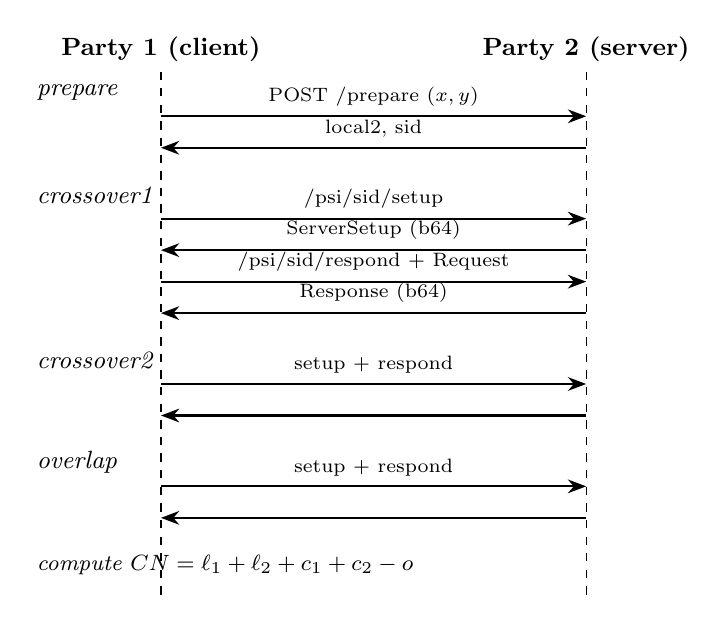
\begin{tikzpicture}[
      node distance=0pt,
      every node/.style={font=\small},
      arr/.style={-Stealth, thick},
    ]
    \node (p1) at (0, 0) {\textbf{Party 1 (client)}};
    \node (p2) at (5.4, 0) {\textbf{Party 2 (server)}};
    \draw[dashed] (p1) -- ++(0,-7.0);
    \draw[dashed] (p2) -- ++(0,-7.0);

    \node[anchor=west, font=\small\itshape] at (-1.7, -0.55) {prepare};
    \draw[arr] (0, -0.85) -- node[above, font=\scriptsize] {POST /prepare $(x,y)$} (5.4, -0.85);
    \draw[arr] (5.4, -1.25) -- node[above, font=\scriptsize] {local2, sid} (0, -1.25);

    \node[anchor=west, font=\small\itshape] at (-1.7, -1.85) {crossover1};
    \draw[arr] (0, -2.15) -- node[above, font=\scriptsize] {/psi/sid/setup} (5.4, -2.15);
    \draw[arr] (5.4, -2.55) -- node[above, font=\scriptsize] {ServerSetup (b64)} (0, -2.55);
    \draw[arr] (0, -2.95) -- node[above, font=\scriptsize] {/psi/sid/respond + Request} (5.4, -2.95);
    \draw[arr] (5.4, -3.35) -- node[above, font=\scriptsize] {Response (b64)} (0, -3.35);

    \node[anchor=west, font=\small\itshape] at (-1.7, -3.95) {crossover2};
    \draw[arr] (0, -4.25) -- node[above, font=\scriptsize] {setup + respond} (5.4, -4.25);
    \draw[arr] (5.4, -4.65) -- (0, -4.65);

    \node[anchor=west, font=\small\itshape] at (-1.7, -5.25) {overlap};
    \draw[arr] (0, -5.55) -- node[above, font=\scriptsize] {setup + respond} (5.4, -5.55);
    \draw[arr] (5.4, -5.95) -- (0, -5.95);

    \node[font=\footnotesize\itshape, anchor=west] at (-1.7, -6.55)
      {compute $\text{CN} = \ell_1 + \ell_2 + c_1 + c_2 - o$};
  \end{tikzpicture}
  \Description{Sequence diagram of one Common Neighbors query. Party 1 first calls POST /prepare with the candidate pair and receives Party 2's local intersection size and a session ID. Three PSI sub-protocols then run, each consisting of a /psi/sid/setup call (returning a base64 ServerSetup) followed by a /psi/sid/respond call (sending a base64 Request and receiving a base64 Response). Party 1 finally combines local and crossover terms.}
  \caption{HTTP message flow for one Common Neighbors query (3 PSI calls = 6 round trips after \texttt{/prepare}). Jaccard adds two further \emph{degree\_x} and \emph{degree\_y} PSI calls.}
  \label{fig:sequence}
\end{figure}

\subsection{Two-Party Jaccard via PSI}
Jaccard is a direct extension of the CN protocol. The numerator is $\text{CN}(x,y)$; each union size is $|N_1(x) \cup N_2(x)| = |N_1(x)| + |N_2(x)| - |N_1(x) \cap N_2(x)|$, and analogously for $y$, giving
\[
J(x,y) \;=\; \frac{\text{CN}(x,y)}{|N_1(x) \cup N_2(x)| + |N_1(y) \cup N_2(y)| - \text{CN}(x,y)}.
\]
Each union adds one PSI call (the degree overlap), and Party 2 must reveal $|N_2(x)|$ and $|N_2(y)|$ in \texttt{/prepare}. Total cost: 5 PSI calls per query and a 2-integer degree leak.

\subsection{Network Layer and Wire Format}
Consumer machines on different networks generally cannot reach each other directly because of NAT, firewalls, and lack of public IPs. We address this with \emph{localtunnel}, a Node.js tool that exposes a local port at a randomly assigned \texttt{*.loca.lt} subdomain. The Streamlit dashboard launches the uvicorn server and tunnel together and prints the public URL; the CLI server (\texttt{pplp-server}) offers a parallel ngrok-based path. Localtunnel interposes a one-time splash page, which the client bypasses by setting the corresponding header. No firewall configuration is required on either side.

OpenMined PSI returns its setup, request, and response messages as protocol buffer objects. JSON cannot carry binary directly, so each is base64-encoded on the wire ($\approx 33\%$ overhead). Because PSI message sizes are dominated by GCS-compressed cryptographic material, this overhead is small in absolute terms (Section~\ref{sec:results}, Table~\ref{tab:perf}).

\subsection{Frontend and Validation}
The Streamlit dashboard provides the web frontend anticipated at midterm. Each party uploads a CSV edge list, selects a role, and either starts the server or supplies a server URL. The same FastAPI endpoints back the dashboard, the Python API, and the test suite.

Correctness is verified against an in-process plaintext baseline. The test suite covers the graph data structure, the local PSI primitive, local CN and Jaccard, the FastAPI server, the HTTP client, and end-to-end remote computation on synthetic graphs. The paper's worked example (Figure~\ref{fig:cn-result}, $|\text{CN}(A,E)|=3$) is one of the test cases, and remote and local results agree.

\subsection{Microbenchmarks}
\label{sec:results}
Table~\ref{tab:perf} reports timing and wire-payload measurements for synthetic graphs in which both candidate nodes have neighborhoods of the listed size. Each row is the median of multiple trials; the FastAPI test client is in-process, so network latency is excluded. Three observations follow:

\begin{itemize}
  \item Local PSI cardinality scales roughly linearly with neighborhood size (3.2 ms at 10 neighbors $\rightarrow$ 161 ms at 1\,000).
  \item Remote CN takes $\approx 3\times$ a single PSI call (3 PSI calls); remote Jaccard takes $\approx 5\times$ (5 PSI calls). The HTTP layer adds 5--15 ms of constant overhead per query.
  \item Wire payload is dominated by the PSI \emph{response} (GCS-encoded ECDH curve points). At a neighborhood size of 1\,000 the average response body is $\approx 47$\,kB; the full CN query transfers $\approx 150$\,kB inclusive of base64 overhead. \texttt{/prepare} bodies are constant ($\approx 113$\,B).
\end{itemize}

\begin{table}[t]
  \centering
  \small
  \caption{Per-query latency and wire payload as a function of per-side neighborhood size $|N(x)|=|N(y)|$. Latencies in milliseconds (median of 3--5 trials), payloads in bytes per HTTP exchange. Apple Silicon, in-process FastAPI test client.}
  \label{tab:perf}
  \begin{tabular}{r r r r r r r}
    \toprule
    & \multicolumn{3}{c}{Latency (ms)} & \multicolumn{3}{c}{Wire (B/call)} \\
    \cmidrule(lr){2-4} \cmidrule(lr){5-7}
    $|N|$ & PSI & CN\textsubscript{rem} & Jac\textsubscript{rem} & prep & setup & resp \\
    \midrule
    10    & 3.2   & 20.8  & 23.3   & 112 & 84    & 643    \\
    50    & 9.4   & 30.0  & 61.5   & 113 & 152   & 2\,854   \\
    100   & 18.7  & 37.9  & 94.0   & 113 & 216   & 4\,750   \\
    500   & 82.0  & 140.0 & 287.6  & 114 & 870   & 23\,667  \\
    1\,000 & 160.5 & 246.0 & 567.3  & 114 & 1\,782 & 47\,283  \\
    \bottomrule
  \end{tabular}
\end{table}

A real wide-area deployment will dominate these numbers with round-trip latency: each CN query costs 7 round trips (1 \texttt{/prepare} + 3$\times$ \texttt{setup} + 3$\times$ \texttt{respond}), and Jaccard costs 11. At a typical 50 ms RTT, that is 350 ms of network time on top of the figures in Table~\ref{tab:perf}.

%=============================================================================
\section{Threat Model in Practice}
%=============================================================================

The semi-honest analysis of Section~\ref{sec:midterm-threat-model} carries over for any single run. Recasting the protocol as a long-lived service (Section~\ref{sec:server-client}) introduces two new threat surfaces the midterm did not consider: adaptive queries against a fixed server graph, and metadata observable through the public tunnel.

\subsection{Adaptive Queries: The Cost of Being a Service}
\label{sec:adaptive-queries}
Demirag/Ayday prove that any single run leaks only intersection sizes; the analysis says nothing about what an adversary learns from a \emph{stream} of carefully chosen queries against a fixed graph. A long-lived server implicitly grants this capability. Three attacks lie outside the prototype's defended threat model:

\begin{itemize}
  \item \textbf{Iterative graph reconstruction.} A malicious client mutates its local graph between queries and observes score changes. Each query reveals one integer, but a few hundred well-chosen queries can recover server-side neighborhoods with high fidelity. The semi-honest analysis does not cover this case: each call is protocol-faithful, but inputs are chosen adaptively across calls.
  \item \textbf{Pair-query oracle.} A malicious client synthesizes a one-edge local graph between two server-side node identifiers of interest. The CN score is then dominated by the server's contribution and effectively reveals whether those two nodes share neighbors on the server side---an edge-presence oracle for any pair the attacker cares about.
  \item \textbf{Malicious-server dual.} A server may substitute a fully connected (or null) graph between Party 1's queries; repeated queries against such manufactured graphs let the server reverse-engineer Party 1's local graph from responses Party 1 trusts.
\end{itemize}

None of these breaks the PSI primitive; they exploit the fact that a queryable service is a function the adversary can invoke repeatedly, and the protocol guarantees nothing about query streams. Defending against adaptive queries is the central open problem our architecture introduces; Section~\ref{sec:future-adaptive} sketches a layered defense.

\subsection{Tunnel-Layer Metadata}
\label{sec:tunnel-leakage}
Routing the server's public reachability through localtunnel introduces a third party that sees every connection. The PSI payload is cryptographically opaque, but four side channels remain. Source IP addresses identify clients (defeating any naive Sybil-resistance scheme that relies only on session state). Request \emph{timing}---in particular the spacing between \texttt{/prepare} and the trailing six (or ten) PSI calls---reliably distinguishes CN from Jaccard queries. Request \emph{sizes} leak the per-call PSI request length, which scales with $|N_1(x)|$ and $|N_1(y)|$ (Table~\ref{tab:perf}); the tunnel can therefore estimate the client's neighborhood sizes per query, which is information the protocol does not authorize. Finally, the JSON envelope itself (endpoint paths, session IDs) is plaintext on the tunnel side. A production deployment should terminate TLS only at the data-holder's own infrastructure, or use a trusted reverse proxy, rather than rely on a free third-party tunnel for transport.

\subsection{Other Out-of-Scope Adversaries}
Collusion among more than two parties, side-channel attacks on the cryptographic library, and active network adversaries (man-in-the-middle on the tunnel beyond the metadata above) are out of scope. A production deployment would additionally need to handle denial-of-service against the in-memory session store and the cost asymmetry of forcing the server to do PSI work per client request.

%=============================================================================
\section{Demo and Use Cases}
\label{sec:demo}
%=============================================================================

We demonstrated the system end-to-end with one server graph and three independent client graphs, mirroring the cross-domain scenarios from Section~1. The server graph is a small social network of ``co-friend'' relationships among the project team and instructors, playing the role of a data-rich provider that wants to monetize query access. Each client holds a bipartite graph drawn from a different domain: Client~1 a user--product retail graph, Client~2 a patient--disease EHR-style graph, and Client~3 a user--show entertainment graph.

Across all four configurations the remote CN and Jaccard outputs agreed exactly with an in-process plaintext baseline computed over the unioned graph, confirming the protocol implementation is correct. Table~\ref{tab:demo} reports representative queries.

\begin{table}[t]
  \centering
  \small
  \caption{Representative queries from the demo. ``Productive'' queries surface latent cross-domain context; ``degenerate'' queries fail predictably. All remote results matched the plaintext baseline.}
  \label{tab:demo}
  \begin{tabular}{l l c c}
    \toprule
    Client & Candidate pair & CN & Jaccard \\
    \midrule
    Retail & (Kaleb\_Kim, Wireless\_Headphones)              & high  & high  \\
    Retail & (Wiam\_Skakri, Mechanical\_Keyboard)            & high  & high  \\
    Retail & (Darin\_Hall, Wireless\_Headphones)             & 0     & 0     \\
    Retail & (Wireless\_Headphones, Mechanical\_Keyboard)    & 0     & 0     \\
    EHR    & (Erman\_Ayday, Goated\_Teaching\_Disorder)      & 0     & 0     \\
    EHR    & (Carson\_Whitehouse, Insomnia)                  & 0     & 0     \\
    EHR    & (Flu, Covid)                                    & 0     & 0     \\
    Shows  & (Wiam\_Skakri, Penguins\_of\_Madagascar)        & high  & high  \\
    Shows  & (Darin\_Hall, The\_Barbie\_Show)                & 0     & 0     \\
    \bottomrule
  \end{tabular}
\end{table}

Three properties characterize productive queries: at least one of $x$ or $y$ is well represented in the server graph, the two graphs share a common node type (e.g., both contain person nodes), and $x$ and $y$ are not already directly connected. Queries that violate any of these---two products, or a pair in which neither node appears on the server---degenerate to local link prediction.

%=============================================================================
\section{Design Tradeoffs}
%=============================================================================

Five tradeoffs shaped the system.

\textbf{Privacy vs.\ efficiency.} The paper's heavier additively-homomorphic variant hides intermediate values from Party 1; we adopted the lightweight variant, accepting a small bounded leakage to avoid FHE round-trips and noise-budget management.

\textbf{Accuracy vs.\ efficiency.} Jaccard yields a more meaningful $0$--$1$ score than raw CN counts but costs 5 PSI calls and reveals two degree sizes (vs.\ 3 calls, no extra leakage for CN). We expose both and let the application choose.

\textbf{Memory vs.\ persistence.} Server-side sessions live in an in-process Python dict with no eviction. Sufficient for a single-process demo; production needs an external store (e.g., Redis) with a TTL.

\textbf{Neighbor counting vs.\ weighting.} CN and Jaccard treat all neighbors equally and map cleanly onto cardinality PSI. Adamic--Adar and Katz weight neighbors by per-node statistics that cardinality PSI does not expose, and need a different primitive.

\textbf{Library portability vs.\ raw PSI speed.} Section~\ref{sec:psi-backend}: we picked ECDH PSI for the pip-installable library. Table~\ref{tab:perf} confirms it is not the bottleneck at our target sizes (hundreds to a few thousand neighbors); for substantially larger graphs the choice should be revisited.

%=============================================================================
\section{System Limitations}
\label{sec:limitations}
%=============================================================================

\textbf{Direct-link disclosure.} If $x$ and $y$ are direct neighbors in Party 2's graph, the paper prescribes an early ``direct link'' abort. We surface this as a \texttt{DirectLinkFound} exception locally but suppress the signal over the network: leaking the early-abort condition to a malicious client would be a free edge-presence oracle. The remote server therefore runs the full protocol regardless.

\textbf{Manual candidate selection.} The API requires the client to nominate $(x,y)$; there is no built-in candidate generator. A client lacking prior knowledge of the joint graph may waste queries on uninformative pairs.

\textbf{Low single-query utility.} CN and Jaccard scores are useful for ranking many candidate pairs; an isolated score is not. The library supports batched calls but lacks a ranking helper.

\textbf{OS support.} OpenMined PSI ships prebuilt wheels for macOS and Linux only. Windows requires WSL2 or Docker.

\textbf{Adamic--Adar.} Not implemented. Cardinality PSI does not expose the per-element degree statistics required.

%=============================================================================
\section{Future Work}
\label{sec:future}
%=============================================================================

\subsection{Defending Against Adaptive Queries}
\label{sec:future-adaptive}
The Demirag/Ayday protocol guarantees per-query privacy, but our system places no bound on what a client learns from an adaptive query stream. The defense is necessarily layered:

\begin{itemize}
  \item \textbf{Per-client query budgets and rate limiting.} The lowest-hanging defense; bounds total leakage in absolute terms.
  \item \textbf{Differentially private answers.} Adding calibrated noise to the CN or Jaccard score trades accuracy for a formal $(\epsilon, \delta)$ bound on what any adaptive sequence reveals. Composes naturally with rate limiting.
  \item \textbf{Query-pattern auditing.} Logging client query graphs and detecting structural signatures of reconstruction attacks is detection rather than prevention, but lets the data owner intervene before substantial leakage.
  \item \textbf{Authenticated, persistent client identity.} Required so the above cannot be bypassed by spinning up fresh sessions; without it, every other defense reduces to a Sybil problem.
\end{itemize}

None of these is a cryptographic guarantee on the footing of the PSI primitive, but together they are the toolkit the threat model actually requires.

\subsection{Other Extensions}
\textbf{Heavier privacy variants.} Adamic--Adar and Katz, listed as candidate measures at midterm, were not delivered: both require per-element neighbor statistics that cardinality-only PSI does not expose. Supporting them privately requires either an FHE protocol over weighted sets or a two-round PSI variant that reveals masked elements. Separately, the paper's heavier additively-homomorphic variant hides intermediate intersection sizes from Party 1 entirely, and could be implemented on top of an existing FHE library (Microsoft SEAL, Pyfhel).

\textbf{Practical extensions.} The current implementation models simple, undirected, single-attribute graphs; weighted edges, directed edges, and typed nodes each require extending the data structures and protocol decomposition. The server loads from CSV at startup; backing it with Neo4j or a NetworkX-on-Postgres store would allow live updates and larger graphs. If \texttt{fastpsi} (or another OKVS+VOLE implementation) acquires Python bindings, the PSI backend is small enough ($\sim$20 LOC) that swapping it in would be straightforward and would reduce per-query latency for large graphs.

%=============================================================================
\section{Conclusion}
%=============================================================================

We delivered the library described in our midterm Expected Output: a Python implementation of the Demirag/Ayday two-party PPLP protocol supporting CN (3 PSI calls) and Jaccard (5 PSI calls), runnable across two machines via FastAPI and localtunnel, and accessible through a Python API, CLI, and Streamlit dashboard. We substituted OpenMined PSI for our originally planned ultra-fast PSI backend (Ling et al.) for portability. End-to-end demonstrations across four datasets confirmed correctness against a plaintext baseline; microbenchmarks show $\le 0.6$\,s per query at neighborhood sizes of 1\,000.

The principal systems contribution is recasting the protocol as an asymmetric server--client service (Section~\ref{sec:server-client}). The paper's symmetric peer framing is cryptographically correct but is not how the technology will be deployed; recasting it as a long-lived data-as-a-service endpoint turns it into something a data owner can actually offer. This packaging also surfaces the most interesting open problem: the protocol guarantees per-query privacy but says nothing about adaptive query streams, and our prototype inherits this gap. Closing it---through per-client budgets, differentially private answers, query-pattern auditing, and authenticated client identity---is the direction we would prioritize over further protocol-level work. The library, documentation, and reproducible demonstrations are open source.

%=============================================================================
\section*{Acknowledgments}
%=============================================================================
This project is conducted for CSDS 356/456. We thank the instructors and the authors of the cited works for the foundations on which we build, as well as the OpenMined community for maintaining a portable PSI implementation that made this prototype possible.

\bibliographystyle{ACM-Reference-Format}
\bibliography{references}

\end{document}
